\chapter{Hasil dan Pembahasan}
\section{Hasil Pengujian}
Setelah melaksanakan pengujian sistem seperti yang telah dibahas pada bab sebelumnya sub bab ini akan memaparkan hasil dari percobaan.
\subsection{Eksistensi Fitur}
%\subsubsection{Pemantauan dan Deteksi}
Pemantauan (aktivitas jantung) dan Deteksi (detak dan aritmia) berhasil dilakukan secara realtime (parameter lainnya, dibahas pada sub bab berikutnya). Berikut perbandingan mode \textit{monitoring} pada sistem di Tugas Akhir ini dengan sistem sejenis lainnya yang berada pada puncak 10 Android Playstore (kata pencarian heart rate) \cite{playstore_heart}.

\begin{table}[H]
	\centering
	\begin{tabular}{|l|L{5cm}|c|L{0.5cm}|L{0.5cm}|L{0.5cm}|L{0.5cm}|L{0.5cm}|L{0.5cm}|L{0.5cm}|L{0.5cm}|}
		\hline
		\rowcolor{gray}
		\textbf{No} & \textbf{Produk} & \textbf{Sen} & \multicolumn{8}{c}{\textbf{Fitur}} \\
		\rowcolor{gray}
		 & & \textbf{sor} & A & B & C & D & E & F & G & H \\
		\hline
		1 & Instant Heart Rate : Heart Rate \& Pulse Monitor & PPG & Y & N & Y & Y & N & Y & N & Y \\
		2 & iCare Health Monitor (BP \& HR) & PPG & Y & N & Y & N & N & Y & N & Y \\
		3 & Heart Rate Monitor(REPS) & PPG & Y & N & Y & Y & N & Y & N & Y \\
		4 & Runtastic Heart Rate Monitor \& Pulse Checker & PPG & Y & N & Y & N & N & Y & N & N \\
		5 & Cardiograph - Heart Rate Meter & PPG & Y & N & Y & Y & N & Y & N & Y \\
		6 & ASUS Heart Rate & PPG & N & N & N & N & N & Y & N & N \\
		7 & Samsung Health & PPG & Y & Y & N & N & N & Y & N & Y \\
		8 & Heart Rate Monitor(Meet Your Need Production) & PPG & N & N & N & N & N & Y & N & N \\
		9 & MobECG & ECG & N & Y & Y & Y & N & Y & N & N \\		
		10 & CMS50Dplus & ECG & N & Y & Y & Y & N & Y & N & N \\
		\hline
		\textbf{*} & \textbf{Tugas Akhir} & \textbf{PPG} & \textbf{Y} & \textbf{Y} & \textbf{Y} & \textbf{Y} & \textbf{Y} & \textbf{Y} & \textbf{Y} & \textbf{Y} \\
		\hline
	\end{tabular}
\end{table}

Ket: \\
A = Identitas User \\
B = Real Time Monitoring \\
C = Melihat Gelombang Jantung \\
D = Merekam Gelombang Jantung \\
E = Multiuser Monitoring \\
F = Deteksi BPM \\
G = Aritmia Alert \\
H = Share Result via Network\\

\subsection{Delay}
Pengujian dilakukan oleh pengguna yang bergerak secara bebas dalam wilayah cakupan router (\textit{receptor}, \textit{router} dan \textit{server} masih dalam satu wilayah) sehingga tidak ada proses routing antara router. Setelah melakukan pengujian sebanyak 3 kali pada waktu berbeda (pagi, siang, malam). Berdasarkan pengujian, didapatkan rata-rata delay percobaan-1 1.60624 ms, percobaan-2 1.36287 ms dan percobaan-3 1.45066 ms. Hasil pengukuran delay tertera pada gambar \ref{fig:delay}. Rata-rata ketiga percobaan ialah 1.47326 ms per sampel.

\begin{figure}[H]
	\centering
	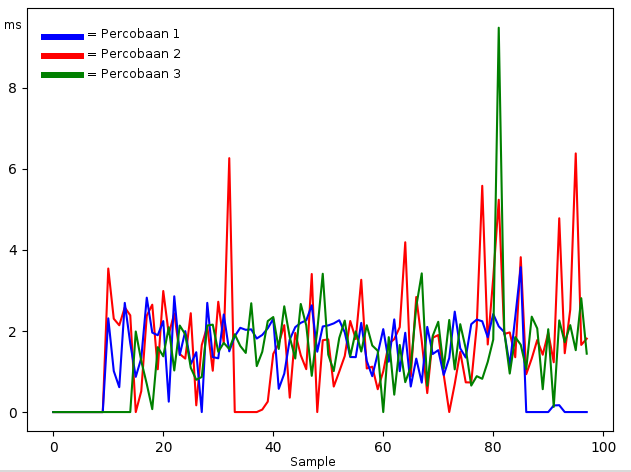
\includegraphics[scale=0.5]{images/delay1.png}
	\caption{Hasil Pengukuran Delay 100 sample}
	\label{fig:delay}
\end{figure}

\subsection{Execution Time}
\textit{Execution Time} perlu diukur pada 2 lokasi yaitu \textit{Receptor} dan \textit{Server}. Hal ini ditujukan untuk mengetahui \textit{maximum sampling speed} yang mungkin dilakukan pada \textit{receptor} sebelum terjadi \textit{bottleneck}. 

Pengujian pada \textit{receptor} dilakukan sebanyak 3 kali pada waktu yang berdekatan (setelah pengujian, \textit{receptor} di \textit{reboot}). Berdasarkan pengujian, didapatkan rata-rata waktu eksekusi percobaan-1 4.36471 ms, percobaan-2 4.74046 ms dan percobaan-3 4.93947 ms. Hasil pengukuran waktu eksekusi tertera pada gambar \ref{fig:exec_time}. Rata-rata ketiga percobaan ialah 4.68155 ms per sampel. Waktu yang berbeda beda ini dipengaruhi oleh adanya \textit{interupt} pengambilan sampel, pembuatan dan pengiriman paket, dan \textit{buffer memory management}. Sebagai perbandingan, tanpa melakukan pengiriman waktu eksekusi hanya selama 0.001 ms (waktu untuk mengambil sampel).

Pengujian pada \textit{server} dilakukan dengan 3 \textit{receptor} yang terhubung (2 + 1 virtual). Berdasarkan pengujian, didapatkan rata-rata waktu eksekusi percobaan-1 0.009496 ms, percobaan-2 0.007823 ms dan percobaan-3 0.008909 ms. Hasil pengukuran waktu eksekusi tertera pada gambar \ref{fig:exec_time2}. Rata-rata ketiga percobaan ialah 0.008742 ms per sampel. Terlihat pada awal waktu eksekusi sangat tinggi kemudian sangat rendah lalu berfluktuasi, hal ini karena pada tahap awal server akan membuka \textit{subprocess} untuk tiap \textit{receptor} yang terhubung. Kemudian, tiap proses hanya mengisi buffer hingga cukup untuk dilakukan operasi deteksi. Penggunaan Node.JS sebagai server juga memberikan 
dampak dalam kecepatan. Dibandingkan dengan Python, Node.JS dapat bekerja hampir 3 kali lebih cepat (gambar \ref{fig:exec_time3}).

\begin{figure}[H]
	\centering
	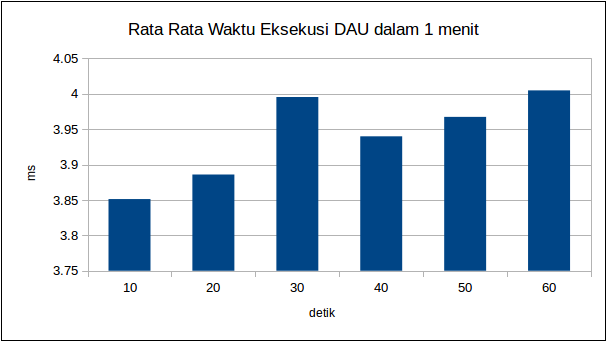
\includegraphics[scale=0.5]{images/exec_time1.png}
	\caption{Hasil Pengukuran Waktu Eksekusi Pada Receptor}
	\label{fig:exec_time}
\end{figure}

\begin{figure}[H]
	\centering
	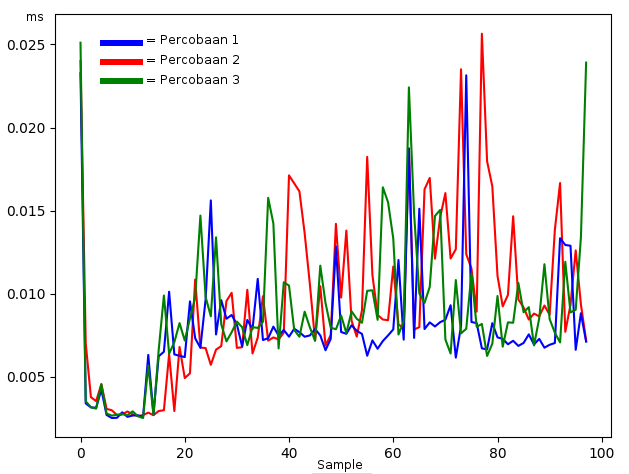
\includegraphics[scale=0.5]{images/exec_time2.png}
	\caption{Hasil Pengukuran Waktu Eksekusi Pada Server}
	\label{fig:exec_time2}
\end{figure}

\subsection{FPS}
Setelah melakukan pengujian, ditemukan FPS terbaik untuk dapat berjalan dengan lancar pada kedua jenis \textit{viewer} yaitu 20 FPS. Hasil lengkap percobaan FPS dapat dilihat pada tabel ...

\begin{table}[H]
	\centering
	\begin{tabular}{|l|l|l|l|}
	
	\end{tabular}
\end{table}

\subsection{Akurasi}
Setelah melakukan pengujian didapatkan hasil akurasi xx\% untuk detaksi detak dan xx\% untuk deteksi aritmia.
\subsubsection{Akurasi Detak}
Dilakukan percobaan untuk menemukan konfigurasi konstanta deteksi $\alpha$, $\beta$ dan $d$ (durasi window).

\begin{figure}[H]
	\centering
	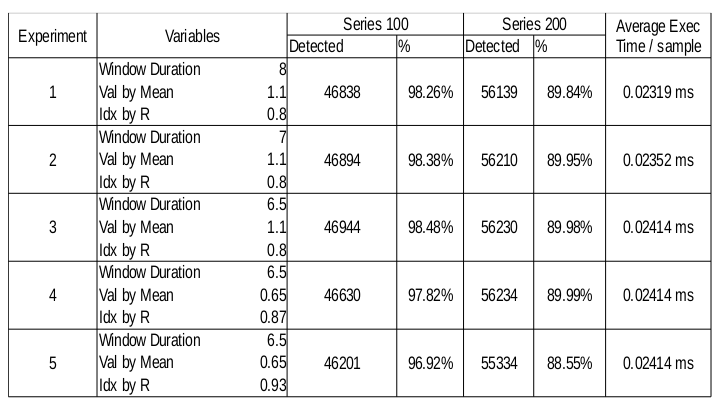
\includegraphics[scale=0.5]{images/exec_time3.png}
	\caption{Hasil Pengujian Algorima Deteksi pada Python}
	\label{fig:exec_time3}
\end{figure}

\subsubsection{Akurasi Aritmia}

\section{Pembahasan}
Dengan terdapatnya mode \textit{monitoring} maka parameter 1 (Eksistensi Fitur) dinyatakan terpenuhi.


\textit{Delay} dan \textit{Execution time} ini terhitung kecil sehingga tidak menyebabkan fenomena \textit{bottleneck} pada sisi server.